\documentclass[10pt,twocolumn]{article}
\usepackage[a4paper,margin=18mm]{geometry}
\usepackage{amsmath,amssymb}
\usepackage{graphicx}
\usepackage{booktabs}
\usepackage[numbers,sort&compress]{natbib}

\title{Lesion-Guided Referral Grading of Diabetic Retinopathy from Fundus Photographs}
\author{Jordan Lee\textsuperscript{1} \and Taylor Morgan\textsuperscript{2} \and Sam Rivera\textsuperscript{1,*}\\
\small\textsuperscript{1}Department of Biomedical Engineering, Example University, Example City, Exampleland\\
\small\textsuperscript{2}Department of Ophthalmology, Example General Hospital, Example City, Exampleland\\
\small\textsuperscript{*}Corresponding author: sam.rivera@example.edu}
\date{}

\begin{document}
\maketitle

\begin{abstract}
Deep learning models can grade diabetic retinopathy from fundus photographs with high accuracy.
However, they rarely show why an image is referred, which limits their acceptance in primary care.
We propose LesionTriage, a two-stage network that first localises lesions and then grades referral urgency from them.
The model was developed on 12,400 colour fundus photographs from two hospitals and tested on 1,850 images from an independent screening programme.
On the external test set, LesionTriage achieved an AUC of 0.94, compared with 0.89 for an image-level classifier.
These results suggest that lesion-level evidence improves both accuracy and trust, supporting its use in community screening.
\end{abstract}

\noindent\textbf{Keywords:} diabetic retinopathy; explainability; referral; fundus photography

\section{Introduction}

Diabetic retinopathy is a leading cause of preventable blindness among working-age adults \citep{morgan2021burden}.
Referral grading is commonly performed by trained human graders, which is time-consuming and subject to inter-observer variability.
Automated screening has therefore attracted increasing attention, especially where specialist graders are scarce.

Previous studies have applied convolutional networks to referral grading and reported sensitivities above 90\% \citep{example2022deep}.
Rivera et al. improved lesion detection by adding a multi-scale attention module \citep{rivera2023attention}.
Despite these advances, explaining the reason for referral remains an open problem.
Most of these models are trained only with image-level labels, so they may rely on camera artefacts rather than the lesions themselves \citep{sample2024shortcut}.

In this study, we aim to make referral decisions traceable to the lesions that justify them.
To this end, we designed a two-stage network that grades referral urgency only from the lesions it detects.

\section{Methods}

This retrospective study included 12,400 colour fundus photographs collected at two tertiary hospitals between 2019 and 2023.
The study was approved by the institutional review board (IRB-0000-00), and the requirement for informed consent was waived because all images were de-identified.
Each image was independently labelled by two certified graders; disagreements were resolved by a senior ophthalmologist.

Fig.~\ref{fig:overview} illustrates the overall pipeline of LesionTriage, which consists of two stages.
The first stage detects haemorrhages, microaneurysms and exudates; the second stage grades referral urgency from the detected lesions.
The network was optimised with a weighted cross-entropy loss, defined as Eq.~(\ref{eq:loss}).

\begin{equation}
\mathcal{L} = -\sum_{c=1}^{C} w_c \, y_c \log \hat{y}_c
\label{eq:loss}
\end{equation}

\begin{figure}[t]
\centering
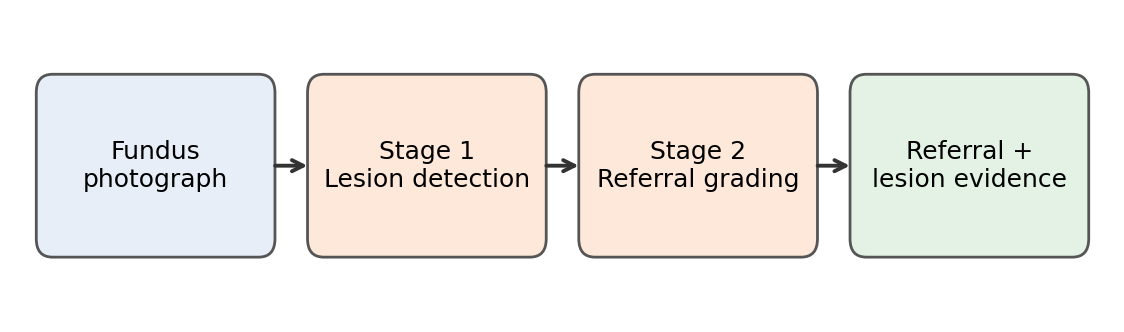
\includegraphics[width=\linewidth]{figures/overview.png}
\caption{Overview of LesionTriage: lesion detection followed by referral grading.}
\label{fig:overview}
\end{figure}

The model was trained for 60 epochs with AdamW, a learning rate of $3 \times 10^{-4}$ and a batch size of 16.
Performance was measured by AUC, sensitivity and specificity, with 95\% confidence intervals from 2,000 bootstrap samples \citep{efron2020bootstrap}.

\section{Results}

LesionTriage outperformed all baselines on the external test set (Table~\ref{tab:main}).
Compared with the image-level classifier, LesionTriage improved sensitivity from 0.86 to 0.92 while keeping specificity above 0.90.
Removing the lesion branch reduced AUC by 0.03, indicating that lesion evidence contributes to the referral decision.

\begin{table}[t]
\centering
\caption{Referral performance on the external test set (95\% CI).}
\label{tab:main}
\begin{tabular}{lccc}
\toprule
Model & AUC & Sensitivity & Specificity \\
\midrule
Image-level classifier & 0.89 & 0.86 & 0.91 \\
LesionTriage w/o lesion branch & 0.91 & 0.88 & 0.90 \\
LesionTriage & \textbf{0.94} & \textbf{0.92} & 0.91 \\
\bottomrule
\end{tabular}
\end{table}

\section{Discussion}

This study shows that grading referral urgency from detected lesions improves accuracy without a separate explanation step.
One possible explanation is that lesion-level supervision discourages the model from using image borders and illumination.
Our findings are consistent with Rivera et al. \citep{rivera2023attention}, who reported that attention to lesions improves generalisation.

This study has several limitations.
First, all images were collected in one country.
Second, lesion annotations were available only for the development set.
Future work will evaluate the system prospectively in community clinics.

\section{Conclusion}

We presented LesionTriage, a referral model that explains its decisions through detected lesions.
LesionTriage may help screening programmes refer patients faster and with greater confidence.


\bibliographystyle{unsrtnat}
\bibliography{refs}
\end{document}
